
% to choose your degree
% please un-comment just one of the following
\documentclass[bsc,frontabs,twoside,singlespacing,parskip]{infthesis} 
\usepackage{graphicx}
%\usepackage{natbib}
\graphicspath{ {images/} }

%	BASIC CRITERIA
%	-	Understanding of the problem
%	-	Completion of the project.
%	-	Quality of the work
%	-	Quality of the report

%	ADDITIONAL CRITERIA
%	-	Knowledge of the literature
%	-	Critical evaluation of previous work
%	-	Critical evaluation of own work
%	-	Justification of the design decisions
%	-	Solution of any conceptual problems
%	-	Amount of work

%	EXCEPTIONAL CRITERIA
%	-	Evidence of originality
%	-	Outstanding scholarship and/or publishable research

\begin{document}

\title{Text Driven Talking Heads}

\author{Iain Brown}
\course{Computer Science}
\project{Undergraduate Dissertation} 
%\project{Undergraduate Thesis} % AI%Psy
%\project{4th Year Project Report}

\date{\today}
%\abstract{The aim of this project is to build a head motion synthesizer for a lifelike animated avatar. The head motions will be predicted entirely from the text of transcribed speech with the aim of finding a mapping between the text and natural head motions. Unlike previous areas of research where the head motions are generated from recorded speech.}
\maketitle
%\section*{Acknowledgements}
%Acknowledgements go here. 
\tableofcontents

% ============================================================= %
\chapter{Introduction}
- Head motion is very important when it comes to human communication\\
- Dialogue is much harder to fully understand without the non-verbal information\\
- Generating Lifelike avatars in many applications, VR, video games, shopping assistant \\
- Realistic head motions are vital otherwise humans may feel weird interacting with an avatar \\
- Project aimed to create a system that synthesises natural head motions just from the text \\
- Without knowledge present in speech\\
- Using Various Natural Language Processing Techniques \\

% ============================================================= %
\chapter{Background Information}

\section{Data and Task}

\subsection{Recordings}
- Participants asked to read fairy tails \\
- Wearing Motion capture software \\
- Recordings transcribed \\

\subsection{Euler Angles}
- Commonly used in robotics \\
- Represent 3 dimensional movements in terms of 3 variables\\

\begin{figure}[h!]
	\caption{Euler Angles in Robotics}
	\centering
	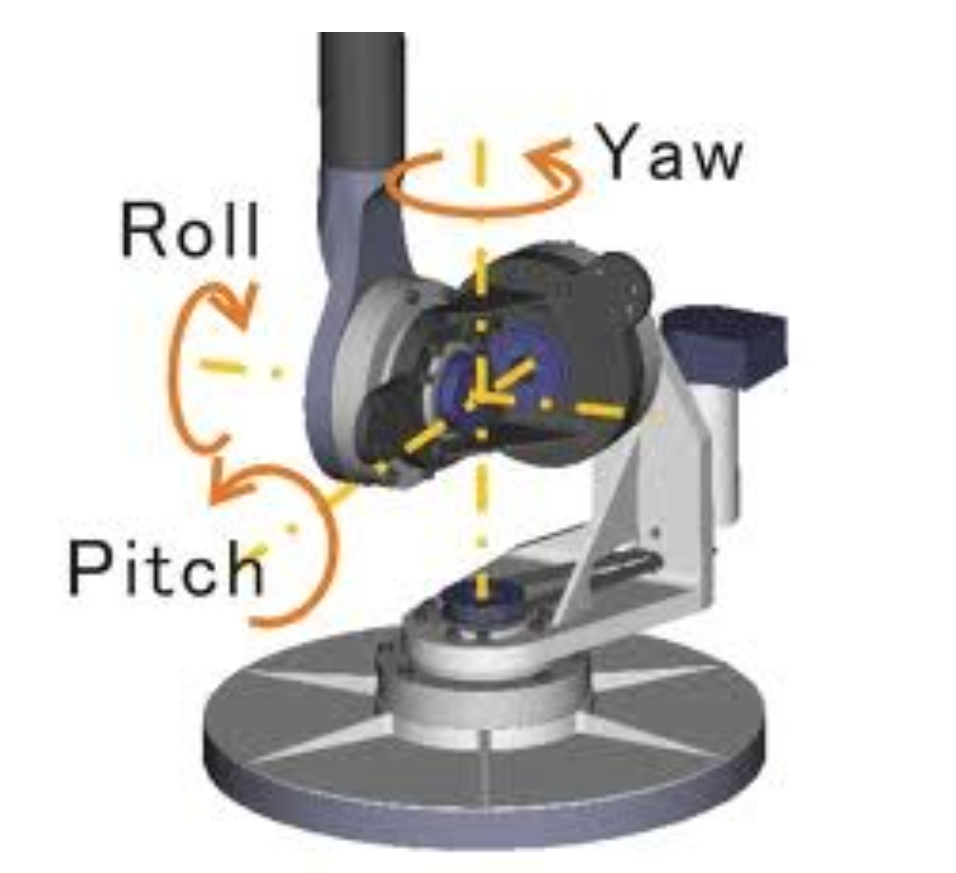
\includegraphics[width=.5\textwidth]{euler_angles.png}
\end{figure}

\subsection{Poser Animation}
- 3D Animation software \\
- Has Python Extension to allow scripting \\
- Euler Angle manipulation \\

% ============================================================= %
\chapter{Text-Driven Head Motion Synthesis}
% This will be the theoretical implementation details 

\section{Hypotheses}
\subsection{Prosodic Features}
\subsection{Speech Content}
\subsection{Phrasing}
\subsection{Sentiment}
\section{Tools}
\subsection{Festival}
\subsection{Poser}


% - To develop a system that is capable of synthesising a life-like talking head from text.
% - use a text to speech system to symnthesize the audio and save data about the audio
% - Build a mapping of words and sentences to discrete head motions
% - Make the system similar to real life (i.e recorded speech)
% - use Poser to animate the head motions
The goal of this project was to develop a system that was capable of synthesising life-like, realistic head motions from transcribed speech. The project aimed to 
\section{Text analysis}
\subsection{Festival}

\section{Head Motion Synthesis}

% ============================================================= %
\chapter{Implementation}

\section{Basic System}

\subsection{Trignomietric Functions}

\section{Random System}

\subsection{Discrete Head Motions}
- Represent Head Motions as discrete N dimensional vectors \\
- Apply smoothing methods to generate overall head shape \\
- Looked into Spherical Linear interpolation \\
- \ cite- people who hiroshi don't like\\

\subsection{Bezier Smoothing}

- Went with Bezier smoothing, similar to SLERP\\
- Bezier Formula
- Bezier doesn't reach the discrete points\\
- This was good for the head motions \\

\begin{figure}
	\caption{Applying Bezier Smoothing to the discrete points}
	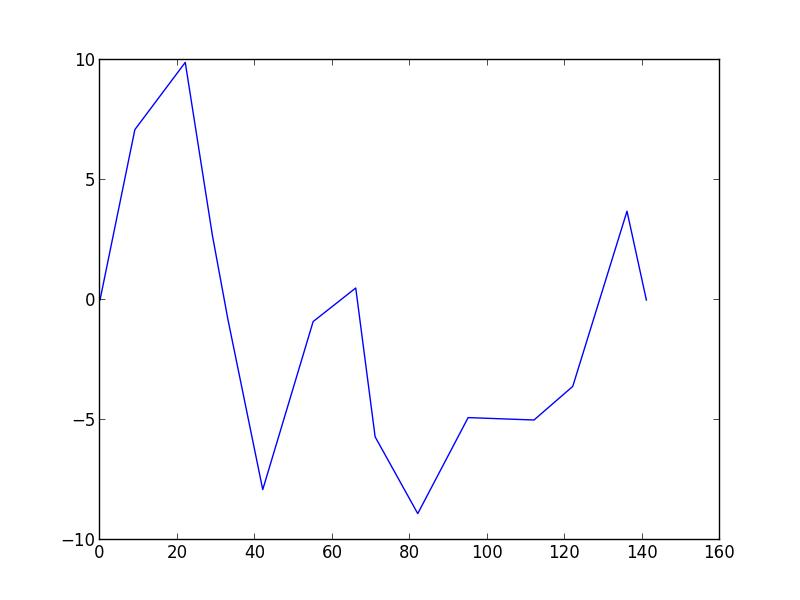
\includegraphics[width=.6\textwidth]{figure_1.png}
	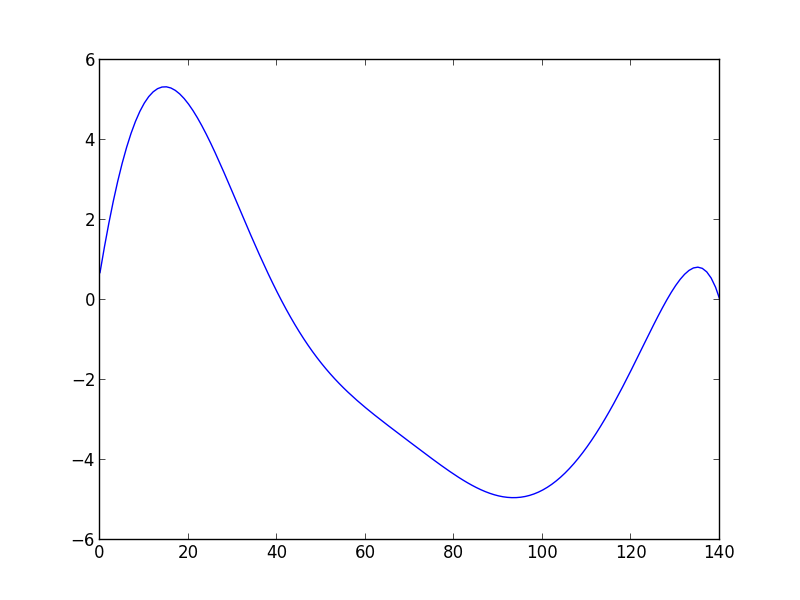
\includegraphics[width=.6\textwidth]{figure_2.png}
\end{figure}

\subsection{Introduction of noise}
- Smoothing was too smooth\\
- Didn't look too natural \\
- Introduced a probability based addition or subtraction\\

\section{Rule-Based System}

\subsection{Parametric Smoothing}
- Felt Bezier did not look like natural head motions \\
- Comparison with data looked too smooth even with noise \\
- Moved towards First Order equations \\
- commonly used in electronics \\
- felt it aligned with recorded head motions more\\
	
% ============================================================= %
\chapter{Evaluation}

To evaluate the Text-Driven Head Motion System I performed both subjective analysis and objective analysis. The aim for the project was to develop a system which generates life-like talking heads with head motions that seem realistic and natural so it was important for humans to evaluate if the head motions were natural or not. Having a unit of measurement describing how close to the original head motions was also necessary in evaluating the system.

\section{Subjective Analysis}

\subsection{Outline}
- Volunteers\\
- 5 Video Clips of animated talking heads \\
- 3 from the TDTH system\\
- 2 taken from actual recordings \\
- All mapped to the same face \\
- Volunteers will be asked to rate on a scale of 1-100 how natural the head motions seem \\
- Focus only on the head motions \\
- Evaluating Only One Criteria
- Not told which are synthesised\\
- Not told about real recordings \\
- So volunteer does not know which were which\\

- Developed Web-based platform for subjective evaluation\\
- Using Python, Flask and HTML5\\
- Used Sliders going from 0-100 \\
- allowed higher precision \\


- Important to keep as much the same as possible\\
- Only change head motions\\
- Apply Dynamic Time Warping\\ 

\subsection{Preliminary Results and feedback}

- Performed evaluation with small number of volunteers \\

- Asked questions about the experience \\
- Difficulty of task \\
- Creepy / Uncanny Valley \\
- Adjust quality of videos \\
- Longer Videos \\ 

\subsection{Results}

- Taken on  board suggestions from preliminary \\
- 15 volunteers \\
- Good results for Random system \\
- Good results for rule-based system \\
- Bad results for ones taken from data \\

\subsection{Conclusions}


\section{Objective Analysis}

- Calculate difference in Euler angles\\
- Compare each system to two recordings due to lack of transcriptions\\

\subsection{Results}
% ============================================================= %
\chapter{Conclusions}

\section{System Overview}

\section{Discussion}
	\subsection{Classification and Regression Trees}
	\subsection{Data Driven System}
\section{Future Work}
	\subsection{Expansion of techniques}
	\subsection{Second Order Smoothing}
	
\bibliographystyle{plain}
\bibliography{diss}

\end{document}
